\documentclass[12pt,a4paper]{article}
\usepackage{graphicx}
\usepackage{geometry}
\usepackage{xcolor}
\usepackage{array}
\usepackage{longtable}
\usepackage{fancyhdr}
\usepackage{amsmath}
\geometry{margin=1in}
\usepackage{array}
\setlength{\headheight}{65pt}
\begin{document}
\noindent

\begin{center}
    \Large\textbf{\color{blue}Gate -PH 2011 46 Question}
\end{center}

\thispagestyle{fancy}
\fancyhf{}
\fancyhead[L]{
\includegraphics[height=1.5cm]{IIITB-COMET-Logo.png}}
\fancyhead[R]{
\begin{tabular}{r}
\textbf{Name:DARSI VAMSI} \\
\textbf{ID: COMETFWC071} \\
\end{tabular}
}
\section*{\color{blue}QUESTION}
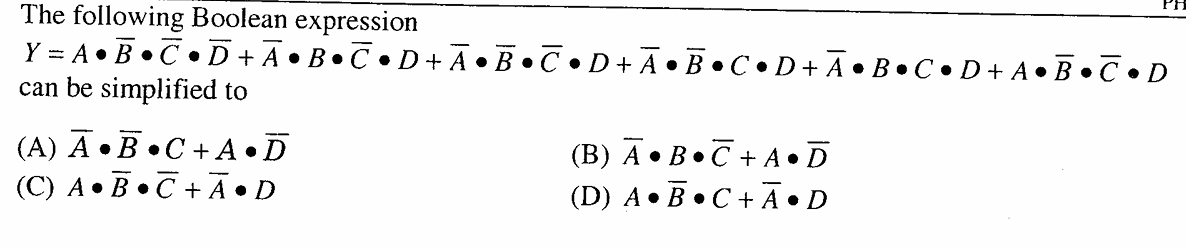
\includegraphics[width=1\textwidth,height=5 cm]{PH 2011 46-esp32.png}
\section*{\color{blue}QUESTION ANALYSIS}
\section*{Solution}
can be simplified to

$$
\begin{array}{ll}
\textbf{(A)}\;
\overline{A}\cdot\overline{B}\cdot C
+
A\cdot\overline{D}
&
\textbf{(B)}\;
\overline{A}\cdot B\cdot\overline{C}
+
A\cdot\overline{D}
\\[0.5cm]
\textbf{(C)}\;
A\cdot\overline{B}\cdot\overline{C}
+
\overline{A}\cdot D
&
\textbf{(D)}\;
A\cdot\overline{B}\cdot C
+
\overline{A}\cdot D
\end{array}
$$

\section*{Solution}

Given,

$$
\begin{aligned}
Y=\;&
A\overline{B}\overline{C}\overline{D}
+\overline{A}B\overline{C}D
+\overline{A}\overline{B}\overline{C}D\\
&+\overline{A}\overline{B}CD
+\overline{A}BCD
+A\overline{B}\overline{C}D
\end{aligned}
$$

\subsection*{Step 1: Group the terms}

Group the first and last terms:

$$
A\overline{B}\overline{C}\overline{D}
+
A\overline{B}\overline{C}D
=
A\overline{B}\overline{C}
(\overline{D}+D)
$$

Since $\overline{D}+D=1$,

$$
A\overline{B}\overline{C}
(\overline{D}+D)
=
A\overline{B}\overline{C}.
$$

Now group the remaining four terms:

$$
\begin{aligned}
&
\overline{A}B\overline{C}D
+
\overline{A}\overline{B}\overline{C}D
+
\overline{A}\overline{B}CD
+
\overline{A}BCD
\\[0.2cm]
&=
\overline{A}D
\left(
B\overline{C}
+
\overline{B}\overline{C}
+
\overline{B}C
+
BC
\right).
\end{aligned}
$$

\subsection*{Step 2: Simplify inside the brackets}

$$
\begin{aligned}
&B\overline{C}
+\overline{B}\overline{C}
+\overline{B}C
+BC
\\[0.2cm]
&=
\overline{C}(B+\overline{B})
+
C(B+\overline{B})
\\[0.2cm]
&=
\overline{C}(1)
+
C(1)
\\[0.2cm]
&=
\overline{C}+C
\\[0.2cm]
&=1.
\end{aligned}
$$

Therefore,

$$
\overline{A}D(1)=\overline{A}D.
$$

\subsection*{Step 3: Final expression}

Hence,


$$
\boxed{
Y=
A\overline{B}\overline{C}
+
\overline{A}D
}
$$

This matches **Option (C).**

$$
\boxed{\text{Correct Answer: (C)}}
$$
\section*{Hardware Components Required}

\begin{table}[h]
\centering
\begin{tabular}{|c|l|}
\hline
\textbf{S.No.} & \textbf{Component} \\ \hline
1 & ESP32-WROOM Development Board \\ \hline
2 & Personal Computer (Ubuntu OS) \\ \hline
3 & USB Cable \\ \hline
4 & Breadboard \\ \hline
5 & LED \\ \hline
6 & 220 $\Omega$ Resistor \\ \hline
7 & Jumper Wires \\ \hline
\end{tabular}
\caption{Hardware and Software Components Required}
\label{tab:hardware}
\end{table}
\section*{Hardware Connections}

\begin{table}[h]
\centering
\begin{tabular}{|c|c|c|}
\hline
\textbf{S.No.} & \textbf{ESP32-WROOM Pin} & \textbf{Connected To} \\ \hline
1 & GPIO 2 & LED Anode (+) \\ \hline
2 & LED Cathode (-) & 220 $\Omega$ Resistor \\ \hline
3 & 220 $\Omega$ Resistor & GND \\ \hline
4 & USB Port & Personal Computer (Ubuntu) \\ \hline
\end{tabular}
\caption{Hardware Connections for LED Interface with ESP32-WROOM}
\label{tab:connections}
\end{table}

\section*{Execution Procedure}

\begin{enumerate}

\item Create a new PlatformIO project for the ESP32-WROOM board.

\begin{verbatim}
/root/venv/bin/pio project init --board esp32dev
\end{verbatim}

\item Place the source code (\texttt{main.cpp}) inside the \texttt{src} directory of the project.

\item Compile the source code and generate the binary files using:

\begin{verbatim}
/root/venv/bin/pio run
\end{verbatim}

\item After successful compilation, the following binary files are generated in the build directory:

\begin{verbatim}
.pio/build/esp32dev/
\end{verbatim}

\begin{itemize}
    \item \texttt{bootloader.bin}
    \item \texttt{partitions.bin}
    \item \texttt{firmware.bin}
\end{itemize}

\item Copy the generated binary files to the desired directory on the Ubuntu PC.

\item Connect the ESP32-WROOM board to the Ubuntu PC using a USB cable.

\item Verify that the ESP32 board is detected by the operating system.

\begin{verbatim}
ls -l /dev/ttyUSB*
\end{verbatim}

\item Verify the ESP32 chip.

\begin{verbatim}
esptool.py --chip esp32 --port /dev/ttyUSB0 chip_id
\end{verbatim}

\item Flash the generated binary files into the ESP32.

\begin{verbatim}
esptool.py --chip esp32 \
  --port /dev/ttyUSB0 \
  --baud 460800 \
  write_flash \
  0x1000 bootloader.bin \
  0x8000 partitions.bin \
  0x10000 firmware.bin
\end{verbatim}

\item Wait until the flashing process completes successfully.

\item Press the \textbf{EN (Reset)} button on the ESP32 board if required.

\item Observe the LED connected to the output GPIO pin to verify the implemented Boolean expression.

\end{enumerate}
\section*{Results and Observations}

The Boolean expression was successfully implemented on the ESP32-WROOM development board. The generated binary files were flashed onto the ESP32 using the \texttt{esptool.py} utility. The output was verified using an LED connected to the output GPIO pin. The LED turned ON for logic HIGH ($Y=1$) and remained OFF for logic LOW ($Y=0$), thereby confirming the correct implementation of the Boolean function.

\subsection*{Truth Table}

\begin{table}[h]
\centering
\begin{tabular}{|c|c|c|c|c|}
\hline
A & B & C & D & Y \\ \hline
0 & 0 & 0 & 0 & 0 \\ \hline
0 & 0 & 0 & 1 & 1 \\ \hline
0 & 0 & 1 & 0 & 0 \\ \hline
0 & 0 & 1 & 1 & 1 \\ \hline
0 & 1 & 0 & 0 & 0 \\ \hline
0 & 1 & 0 & 1 & 1 \\ \hline
0 & 1 & 1 & 0 & 0 \\ \hline
0 & 1 & 1 & 1 & 1 \\ \hline
1 & 0 & 0 & 0 & 1 \\ \hline
1 & 0 & 0 & 1 & 1 \\ \hline
1 & 0 & 1 & 0 & 0 \\ \hline
1 & 0 & 1 & 1 & 0 \\ \hline
1 & 1 & 0 & 0 & 0 \\ \hline
1 & 1 & 0 & 1 & 0 \\ \hline
1 & 1 & 1 & 0 & 0 \\ \hline
1 & 1 & 1 & 1 & 0 \\ \hline
\end{tabular}
\caption{Truth Table of the Implemented Boolean Expression}
\label{tab:truth}
\end{table}

\subsection*{Experimental Output}

Figure~\ref{fig:led_off} shows the LED in the OFF state corresponding to logic LOW ($Y=0$). Figure~\ref{fig:led_on} shows the LED in the ON state corresponding to logic HIGH ($Y=1$).

\begin{figure}[h]
\centering
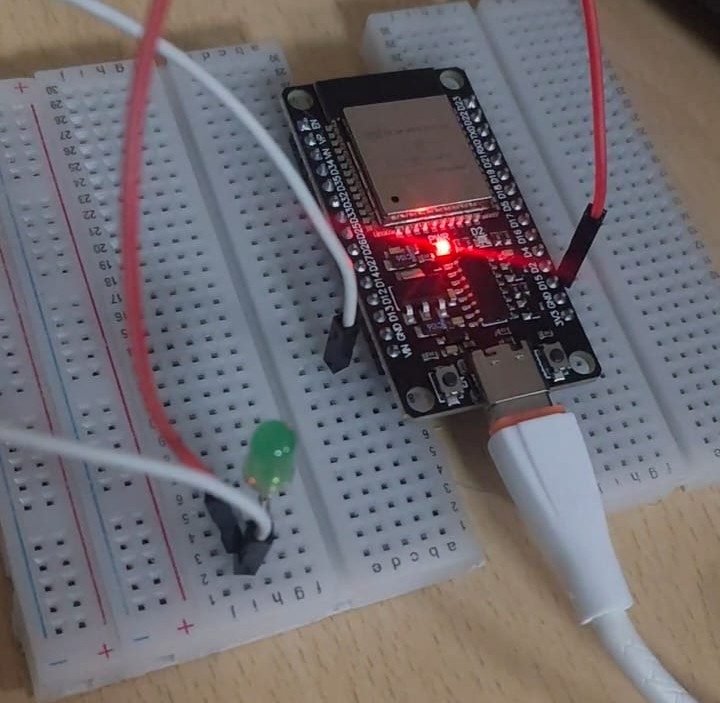
\includegraphics[width=0.45\textwidth]{led_off.jpeg}
\caption{LED OFF (Logic 0)}
\label{fig:led_off}
\end{figure}

\begin{figure}[h]
\centering
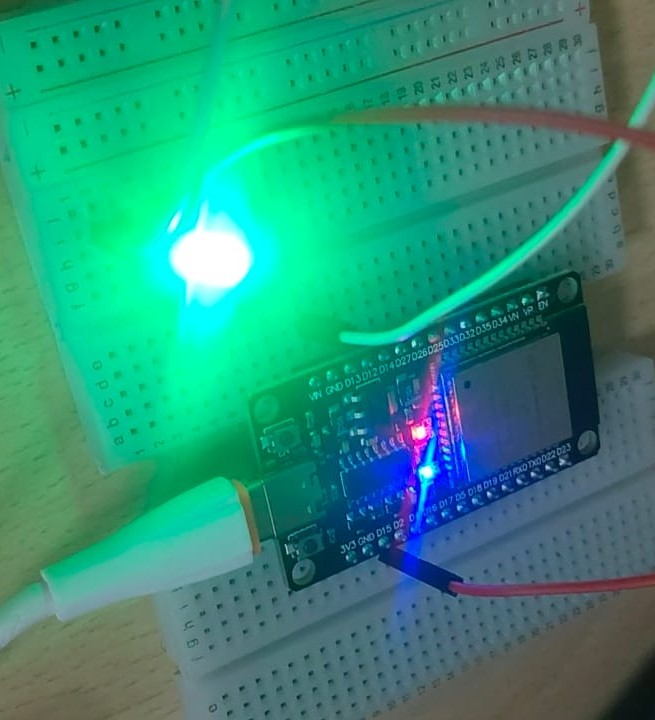
\includegraphics[width=0.45\textwidth]{led_on.jpeg}
\caption{LED ON (Logic 1)}
\label{fig:led_on}
\end{figure}

\subsection*{Result}

The Boolean expression was successfully implemented and verified on the ESP32-WROOM development board. The observed LED output matched the expected truth table for all input combinations.
\end{document}